


% ######################################################################### %
% ------------------------------------------------------------------------- %
%                                Rewiring
% ------------------------------------------------------------------------- %
% ######################################################################### %


\section{Rewiring}\label{sec:rewiring}

% In the network configuration introduced in
% section~\ref{sec:network_model} strong directional anisotropy is
% present: Edges originating from one node \enquote{point in the same
%   direction}, that is they connect to other nodes which cluster around
% a. In this section we introduce an algorithm


% It is in our highest interest to compare results to. 
% %------------------------------------------------
% \marginpar{eliminate anisotropy to find structures connected to it} 
% %------------------------------------------------ 
% To this end we introduce an algorithm that preserves
% distance-dependent connectivity as found in
% Proposition~\ref{distance_prof}, but eliminates anisotropy in network
% connectivity by consecutively rewiring existing connections to new
% suitable targets.


Distance-dependency as identified in the last section may already
account for many of the structural features present in anisotropic
networks. A central question of this study is: What structural aspects
in the network are truly features of the anisotropy in connectivity?
Although a quantitative measure for anisotropy will only be introduced
in the next section, already here we are able to qualitatively observe
the strong directionality in connectivity - edges originating from one
node \enquote{point in the same direction}, effectively aligning with
the orientation of the axonal projection of the source node
(cf. \autoref{fig:anisotropic_network_model}). 
%------------------------------------------------
\marginpar{eliminate anisotropy to find structures caused by it} 
%------------------------------------------------ 
To answer the question above, we need to introduce a method that
eliminates this directionality, making networks essentially isotropic
in connectivity. Then, structural features present in the original
anisotropic networks, but not in their rewired, isotropic counterparts
may be attributed to anisotropy.

Rewiring as introduced here, provides the transition from anistropic
connectivity to networks isotropic in connectivity, closely resembling
purely distance-dependent networks. Applying this process only
partially then allows us to analyse structural features as they change with
a varying degree of isotropy, asserting the importance of this process
to our study. In designing the specific rewiring algorithm we identify
two requirements that our implementation should satisfy: 
%\vspace{-3pt}
\begin{enumerate}
  \itemsep-11pt
  \item elimination of anisotropy in connectivity 
  \item preservation of distance-dependent connectivity
\end{enumerate}
%\vspace{-3pt}%
The second point is especially important to us, as we want to impose
isotropy on the network at \enquote{minimal cost}, that is by changing
as little as possible about the other characteristics of the network's
connectivity. The following process respects both of the points above:
\begin{blockquote}{
For every edge between vertices $v$ and $v'$ with inter-vertex
distance $x$, identify neurons with distance to $v$ in the range of
$(x-\varepsilon, x+\varepsilon)$ as potential new targets. Then pick
at random one of these vertices (including $v'$) as a new target for
the current edge, if such an edge doesn't already exist
(\autoref{fig:distance_rewiring}).}
\end{blockquote}
In the graph theoretic context we
formally define a rewiring as follows:

\vspace{0.2cm}
\begin{figure}[H]
  \centering 
  \makebox[0.875\textwidth]{%
    %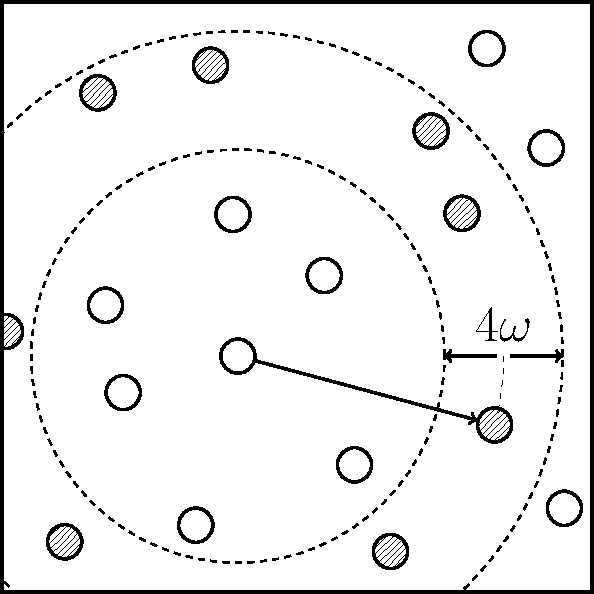
\includegraphics[width=0.4\textwidth]{dist_rew_org.pdf}%
    \begin{overpic}[width=0.4\textwidth, frame]{%
        tikz/distance_rewire_L3.pdf}
      \put(2,102){\small{Before}}
    \end{overpic}
    \hfill
    \begin{overpic}[width=0.4\textwidth, frame]{%
        tikz/distance_rewire_L4.pdf}
      \put(2,102){\small{After}}
    \end{overpic} 
  }%
  \caption{\textbf{Rewiring transforms anisotropic geometric graphs to
      networks with isotropic connectivity} For a given edge $e$ with
    a distance $x$ from its source vertex $v$ to its target vertex
    $t(e)$, potential new targets (striped) are found in within a
    distance $(x-\varepsilon, x+\varepsilon)$ of $v$. The rewired edge
    then projects from $v$ to a new target $t'(e)$, randomly chosen
    from the set of vertices within in this range. Inter-vertex
    distance between $v$ and $t'(e)$ differs by less than
    $\varepsilon$ from $x$, ensuring that for small $\varepsilon$ the
    original distance-dependent connectivity is preserved. (Note that
    all targets within range are eligible for rewiring as no other
    edges exist. In general this is not the case.)}
  \label{fig:distance_rewiring}
\end{figure}


\begin{definition}
  \label{def:rewiring}
  Let $G$ be an anisotropic geometric graph with $\abs{V(G)} =
  n$. Then we define a \textit{rewiring} of $G$ to be probability space over
  $G^n_{\Phi}$, induced by the following process: For every edge $e
  \in E(G)$ uniformly at random pick a potential new target $t'(e)$
  from the set $M_e = T_e \setminus K_e$, where $T_e$ is the set of all
  vertices that differ in their distance to $s(e)$ less than
  $\varepsilon$ from the distance of $s(e)$ to $t(e)$,
  \[ 
  T_e = \left\{v \in V(G) \setminus s(e) \mid \abs{\mathrm{d}(s(e),v)
      - \mathrm{d}(s(e),t(e))} < \varepsilon \right\} %?? definition
                                %of distance d?
  \]
  and $K_e$ the set vertices that already are connected to $s(e)$ by
  another rewired edge, 
  \[
  K_e = \left\{v \in V(G) \mid \exists\, e' \in E'(G): s(e') = s(e),
      t(e') =v \right\},
  \]
  where $E'(G)$ is the set of all edges that have been rewired already.
\end{definition}

Note that in the way Definition~\ref{def:rewiring} is formulated, it
is possible for $M_e$ to be empty for some edge $e$. In this case no
new edge is realized and the resulting, rewired network has
$\abs{E(G)}-1$ edges. In practice this happens negligibly seldom, out
of approximately on average only $25.68$ edges, with a standard deviation
of $4.51$ and accounting for roughly $0.02\%$ of the rewired edges, are \enquote{lost}
in this process (\smtcite{4afc2727}). 

We formulated Definition~\ref{def:rewiring} in such a way, that
distance-dependent connectivity is preserved. We verify this claim by the
following estimation:

Let $\tilde{C}(x)$ be the distance-dependent connectivity profile of a
rewiring $R_{\varepsilon}$ of an anisotropic graph $G_{n,w}$. Denote
with $C(x)$ the distance-dependent connection probability of the
$G_{n,w}$. The expected value for $\tilde{C}(x)$ at any point $x$ We
estimate the expected difference between $\tilde{C}(x)$ and $C(x)$ at
any point $x$ as
\begin{align}
  \mathbf{E}\left[\tilde{C}(x) - C(X)\right]  
    & = \int_{x-\varepsilon}^{x+\varepsilon} f(x') C(x') \, dx -
        C(x)\notag\\
    & = \frac{1}{2\varepsilon}\int_{x-\varepsilon}^{x+\varepsilon}
        C(x') - C(x) \, dx \notag\\
    & = \frac{1}{2\varepsilon} \left\{ \int_{x-\varepsilon}^{x} C(x') -
        C(x) \, dx - \int_x^{x+\varepsilon} C(x') - C(x) \, dx
        \right\} \notag\\
    & = \frac{1}{2\varepsilon} \label{eq:rewiring_est}
\end{align}

The rewiring margin $\varepsilon$ thus simultaneously governs how many
new targets are available for each edge and how well
distance-dependency is preserved. Setting $\varepsilon = 1.25$ %??
                                %right value check!
and applying the rewiring algorithm to the 25 sample graphs, we find
that distance-dependent connectivity of the original graphs is matched
(\autoref{fig:rewiring_dst_prf_compare}) while at the same time
ensuring that for any edge $e$ sufficiently many new rewiring targets
are available (\autoref{suppfig:rew_stats}).

\begin{figure}[H]
  \centering
  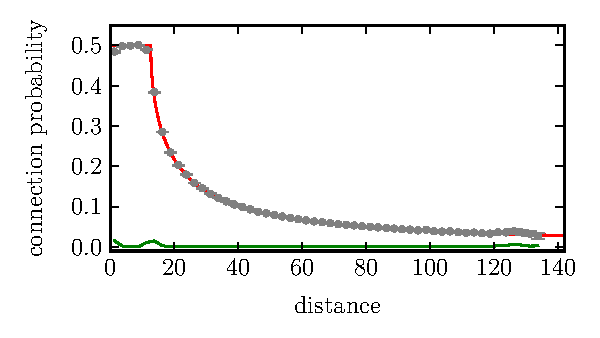
\includegraphics[width=0.8\linewidth]{%
    plots/4f4dfcf1.pdf} 
  \captionsetup{skip=0pt}
  \caption{\textbf{Rewiring with \boldmath$\varepsilon = 1.25$
      preserves distance-dependent profile in sample graphs} Comparing
    the distance-dependent connection probabilities of the original
    graph (Theorem~\ref{theorem:distance_prof}) in red with extracted
    of probabilities from the rewired ($\varepsilon = 1.25$) sample
    graphs in gray (errorbars SEM) we verify that distance-dependent
    connectivity is preserved when rewiring. The green curve shows the
    expected difference between the original and rewired
    distance profiles as estimated in
    Equation~\ref{eq:rewiring_est}. (\smtcite{4f4dfcf1})}
  \label{fig:rewiring_dst_prf_compare}
\end{figure}


As a generalization of Definition~\ref{def:rewiring}, we define a
partial rewiring $R_{\varepsilon, \eta}$, finding new targets only for
a fraction $\eta$ of all edges:

\begin{definition}Let $\varepsilon > 0$ and $0 \leq \eta \leq 1$. A
  \textit{partial rewiring} $R_{\varepsilon,\eta}$ of an anisotropic
  geometric graph $G_{n,w}$ is then a rewiring $R_{\varepsilon}$ of
  $G_{n,w}$, in which every edge is rewired with a probability of
  $\eta$, otherwise it remains. To avoid the occurrence of multiple
  edges, $K_e$ is then extended to include the targets of all edges
  originating from $s(e)$ that will not be rewired.
\end{definition}






 

% \begin{algorithm}
% Let $N(n,e,w) = (G,P,a)$ be  Then 
% \normalfont
% \begin{algorithmic}%[1] <-- gives line numbers
% \For {$v \in V(N_G)$}
%   \For {$e \in E_{\textrm{out}}(v)$}
%      \State $x \gets \norm{N_P(v)-t(e)}$
%      \State $T \gets \{w \in V(N_G) \mid  x-\varepsilon \leq
%      \norm{N_P(v)-N_P(w)} < x+\varepsilon\}$
%      \State $t(e) \gets \textrm{choice} T$
%   \EndFor
% \EndFor
% \end{algorithmic}
% is defined.
% \end{algorithm}


%%% Local Variables: 
%%% mode: latex
%%% TeX-master: "../dplths_document"
%%% End: 
